%
%	Praxisbezug
%

\pagebreak
\section{Data Analysis}

\onehalfspacing

\subsection{Page Impressions}

Unlike Plausible\footnote{See \textit{Frank, C. (2021)}: Web Traffic Analysis - Predicting Blog Post Performance. \cite{previousBigData}}, wp-statistics does not offer detailed measurements for interaction or click-through rates; we'll need to extrapolate some data and behavior from our knowledge of the site.

Let's first look at the anatomy of the blog:

\begin{figure}[H]
\centering
\caption {Page Types}
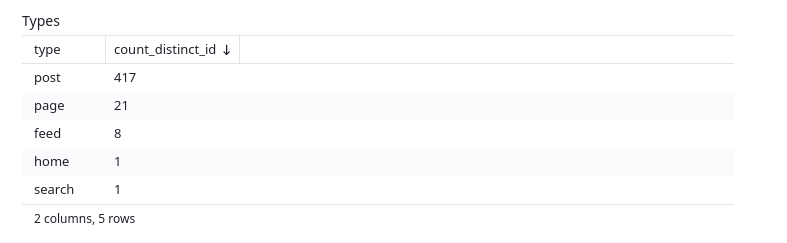
\includegraphics[width=\linewidth]{images/figure10.png}
\label{fig:pageTypes}
\end{figure}

We have 417 separate posts on the blog, and 21 pages, in addition to the home page where people start browsing when they do not come from a search engine or a social media reference. 

The pages are the top-level menu of the blog, and we can ignore them from here on. Also, we will not focus on the RSS Feed or the search function.

We'll now look at the page impressions by type:

\begin{figure}[H]
\centering
\caption {Impression by Page Type}
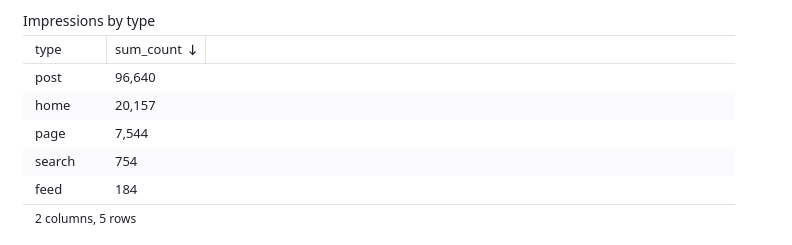
\includegraphics[width=\linewidth]{images/figure11.png}
\label{fig:impressionType}
\end{figure}

The most read items on the blog are the individual posts, which is good for us. It sounds more evident than it is - if a user accesses the main page and scrolls down, we have no way of finding out which post they might have read.

We'll focus on the page impressions of the posts alone and ignore the other types in further analysis.

Let's try to find the top 12 most-read posts:

\begin{figure}[H]
\centering
\caption {Top Performing Posts}
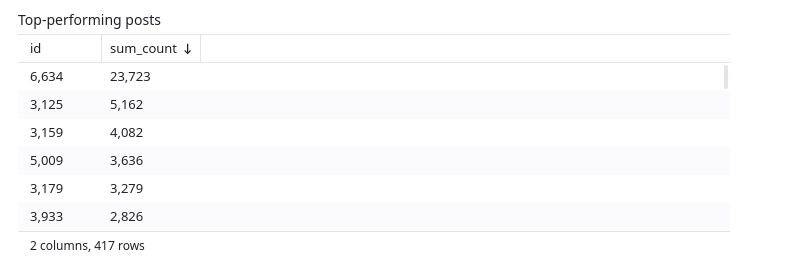
\includegraphics[width=\linewidth]{images/figure12.png}
\label{fig:topPerforming}
\end{figure}

Identifying the actual posts is a bit of manual work: wp-statistics, unfortunately, records in the URI all Url-parameter, including tracking parameters such as fbclid - there's an option in wp-statistics to disable that behavior, but not retroactively. Also, wp-statistics does not record the post title itself. 

Manual review it is!

\begin{figure}[H]
\centering
\caption {Top Performing Posts}
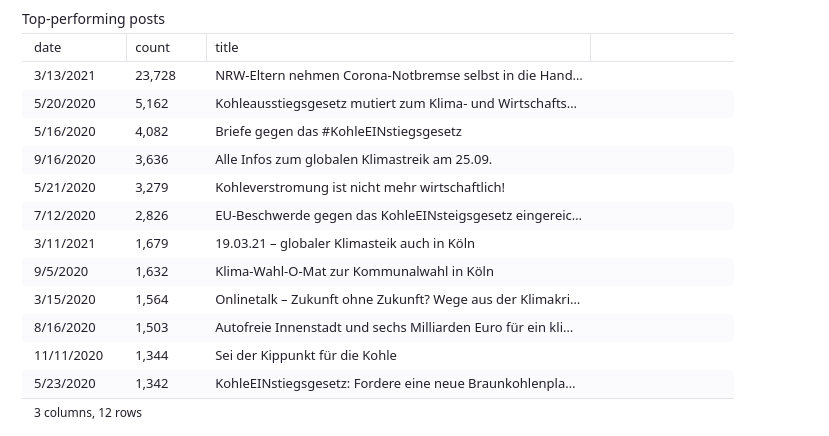
\includegraphics[width=\linewidth]{images/figure13.png}
\label{fig:manualReview}
\end{figure}

In addition to the global climate strike and local elections that we have identified previously, we've now identified the top-performing post related to Covid-19. Not surprisingly.

The next set of lessons learned from the data is that these are best performing subjects:

\begin{itemize}
 \item Covid-19
 \item Local election
 \item Climate strike
 \item Stop fossil fuels
\end{itemize}

The blog is an integral part of the communication and supports the community of climate activists in Cologne.

\subsection{Direct Engagements through Forms}

The blog has a contact form and a donation form. Are people using it?

\begin{figure}[H]
\centering
\caption {Engagement through Forms}
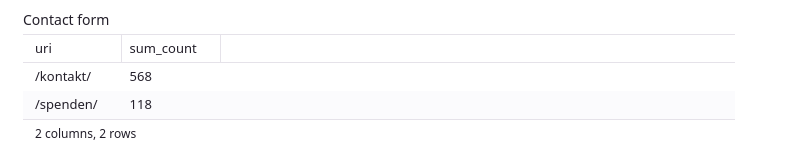
\includegraphics[width=\linewidth]{images/figure14.png}
\label{fig:engagementForms}
\end{figure}

Compared to the posts, these numbers are not impressive. Looking at the pages, lessons learned from this would be:

\begin{itemize}
 \item Redesign contact form
 \item Redesign donations
\end{itemize}

\subsection{Direct Engagement through Comments}

WordPress allows two forms of direct engagement: pingbacks\footnote{See \textit{WPBeginner (2021)}: What is Pingback. \cite{pingBack}} and comments. We do not have any insight into the other form of interaction, trackbacks.\footnote{See \textit{WPExplorer.com (2020)}: WordPress Pingbacks and Trackbacks. \cite{trackBack}}

Let's start with the pingbacks:

\begin{figure}[H]
\centering
\caption {Pingbacks}
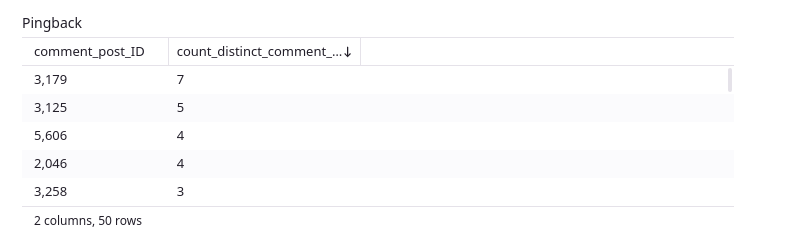
\includegraphics[width=\linewidth]{images/figure15.png}
\label{fig:pingbacks}
\end{figure}

The two most linked posts are also in the list of the dozen most-visited posts and deal with the urgent need to stop using fossil fuels:

\begin{figure}[H]
\centering
\caption {Pingback Targets}
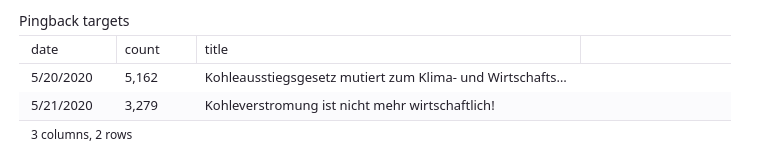
\includegraphics[width=\linewidth]{images/figure16.png}
\label{fig:pingbackTargets}
\end{figure}

Let's continue with the comments:

\begin{figure}[H]
\centering
\caption {Comments}
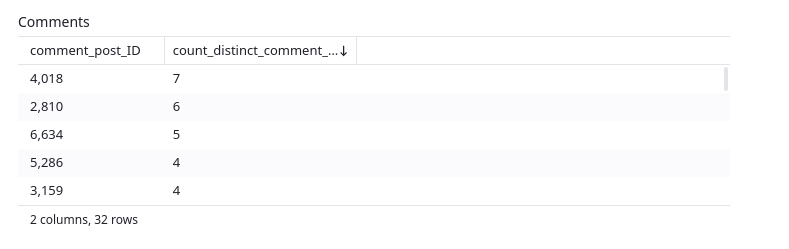
\includegraphics[width=\linewidth]{images/figure17.png}
\label{fig:comments}
\end{figure}

The two posts with the most comments are about participating in  the climate pact and a lignite complaint, and the third is our most visited post:

\begin{figure}[H]
\centering
\caption {Comment Targets}
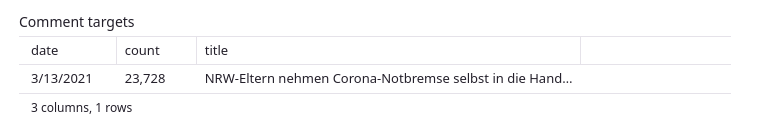
\includegraphics[width=\linewidth]{images/figure18.png}
\label{fig:commentTarget}
\end{figure}

There's significant engagement in our core messages from the community; the blog is an integral part of our digital outreach and helps us keep the activism alive in the Covid-19 pandemic.

As the final step, we'll look at multiple interactions, i.e. comments to comments

\begin{figure}[H]
\centering
\caption {Comments on Comments}
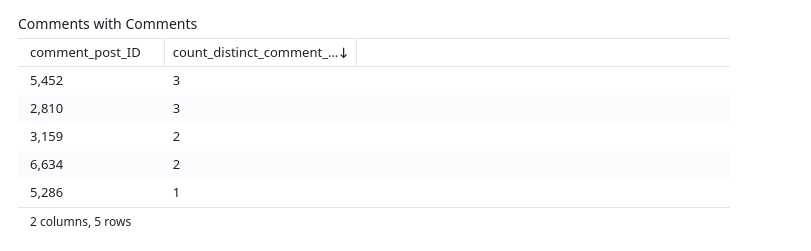
\includegraphics[width=\linewidth]{images/figure19.png}
\label{fig:commentsComment}
\end{figure}

For a blog, this is the highest form of interaction, a post that's not only read and commented on but where the readers have replied to a previous comment! 

\subsection{Improving Analytics}

Improve analytics through the use of Matomo or Plausible

In a previous paper, I have covered Plausible in more detail and compared it with other web analytics tools.\footnote{See \textit{Frank, C. (2020)}: Usefulness of open-source tools for web analytics in E-Marketing. \cite{previousPaper}} I will not go any further into details of the tool itself in this paper. As we will see later, it would be a good alternative to wp-statistics, which is used for the KFF blog

\begin{figure}[H]
\centering
\caption {Plausible}
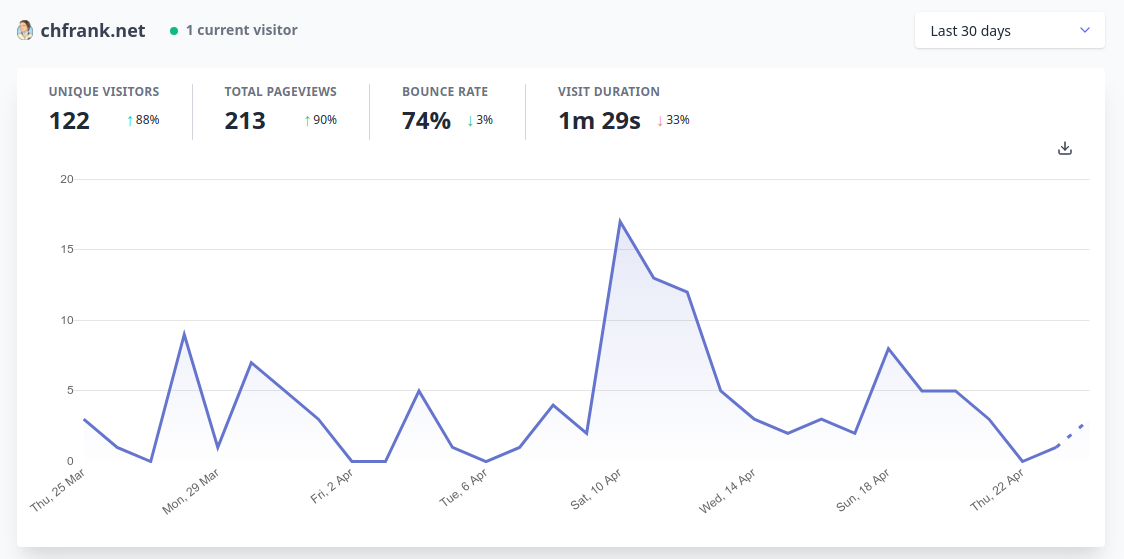
\includegraphics[width=\linewidth]{images/plausible.png}
\label{fig:plausible}
\end{figure}

Pay attention to web vitals\footnote{See \textit{Sousa, B. (2021)}: Google Web Vitals best practices for single-page apps.\cite{webVitals}}

Install a caching plugin to speed up mobile access\footnote{See \textit{Crowe, A. (2021)}: WordPress Checklist. \cite{wpCachePlugin}}

\subsection{Sustaining Engagement}

High community engagement with a focus on local events

Digital activism supports offline activism and can combat loneliness

We need to fight hate speech, Ableism and other forms of -isms in our communication

To improve outreach, implement the lessons learned (IP addresses, data processing info, best-performing subjects, target audience, simplify contact and donations)

Coming back to the original question for the paper "On which subject(s) should I post to increase my reach?" we now have a definite answer.

According to the data, posting more content on Climate Change and Covid-19 should lead to more visitors' engagement.

I'll keep that in mind for the future and change the content that I post accordingly.

Cross-posting to Facebook is an already established automated procedure, so I'll keep doing that for now. Also, I like posting in English, so I'll continue this practice as well.

I will work on the other two recommendations to improve Google search and mobile usability.
